\chapter{Relations Among Trigonometric Ratios}
\label{chap:relations_among_trigonometric_ratios}

\section{Six Trigonometric Relatives}
\label{sec:six_trigonometric_relatives}

So far, we've only seen the following trig functions: \textit{sine, cosine,}
and \textit{tan}. Now, it's time to see the rest of the trig functions.

\begin{figure}[htpb]
	\centering

	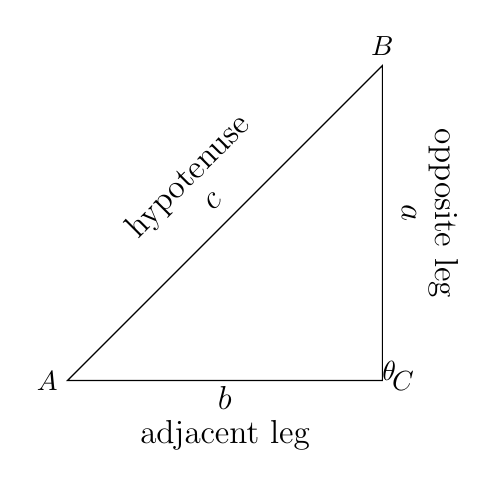
\begin{tikzpicture}
		\coordinate [label=left:$A$] (A) at (-4,0);
		\coordinate [label=above:$B$] (B) at (0,4);
		\coordinate [label=right:$C$] (C) at (0,0);

		\draw (A) -- node[label={[align=center,rotate=45] \large hypotenuse \\ \large $c$}] {}
		(B) -- node[right,label={[align=center,rotate=-90] \large opposite leg \\ \large $a$}] {}
		(C) -- node[below,label={[align=center,label distance=-1cm] \large $b$ \\ \large adjacent leg}] {}
		cycle;

		\tkzMarkAngle[size=0.6cm](C,A,B)

		\tkzLabelAngle(C,A,B){$\theta$};
	\end{tikzpicture}

	\label{fig:right_triangle_named_on_all_sides_using_symbols_and_text}
\end{figure}

In any right triangle, we have a total of $6$ ratios. We've already named $3$ of the $6$
\begin{align*}
	\sin(\theta) = \frac{\textrm{opp}}{\textrm{hyp}} = \frac{a}{c}, \qquad \cos(\theta) = \frac{\textrm{adj}}{\textrm{hyp}} = \frac{b}{c}, \qquad \tan(\theta) = \frac{\textrm{opp}}{\textrm{adj}} = \frac{a}{b}
	.\end{align*}

Now, let's define the next $3$.

\begin{definition}[Cotangent]
	\label{def:cotangent}

	\textbf{Cotangent} is a trigonometric function of an angle that calculates
	the ratio of the adjacent side divided by the opposite side of the angle as
	follows
	\[%
		\cot(\theta) = \frac{\textrm{adj}}{\textrm{opp}} = \frac{b}{a}
  .\]%
\end{definition}

\begin{definition}[Secant]
	\label{def:secant}

	\textbf{Secant} is a trigonometric function of an angle that calculates
	the ratio of the hypotenuse divided by the adjacent side of the angle as
	follows
	\[%
		\cot(\theta) = \frac{\textrm{hyp}}{\textrm{adj}} = \frac{c}{b}
  .\]%
\end{definition}

\begin{definition}[Cosecant]
	\label{def:cosecant}

	\textbf{Cosecant} is a trigonometric function of an angle that calculates
	the ratio of the hypotenuse divided by the opposite side of the angle as
	follows
	\[%
		\cot(\theta) = \frac{\textrm{hyp}}{\textrm{opp}} = \frac{c}{a}
  .\]%
\end{definition}

\subsection{Reciprocal Functions}
\label{sub_sec:reciprocal_functions}

\begin{definition}[Reciprocal Fractions]
	\label{def:reciprocal_fractions}

	\textbf{Reciprocal fractions} are fractions that represent $\frac{1}{x}$ of a
	given quantity of $x$. When multiplied by $x$, they give the product of $1$.
\end{definition}

\begin{example}
	\label{exm:reciprocal_fractions}

	The reciprocal fraction of $\frac{1}{5}$ is $5$ because $\frac{1}{5} \times 5 = 1$
\end{example}

Let's look at all $6$ trigonometric functions, where $a$ and $b$ are the
lengths of the triangle's legs and $c$ is the length of the hypotenuse
\[%
	\sin(\theta) = \frac{a}{c}, \cos(\theta) = \frac{b}{c}, \tan(\theta) = \frac{a}{b}, \cot(\theta) = \frac{b}{a}, \sec(\theta) = \frac{c}{b}, \csc(\theta) = \frac{c}{a}
.\]%

The cotangent is the reciprocal of the trangent, the cosecant is the reciprocal
of the sine, and the secant is the reciprocal of the cosine.

You can summarize these facts by expressiong them as
\[%
	\cot(\theta) = \frac{1}{\tan(\theta)}, \csc(\theta) = \frac{1}{\sin(\theta)}, \csc(\theta) = \frac{1}{\cos(\theta)}
.\]%

These formulas are helpful when proving trigonometric identites.

\begin{definition}[Trigonometric Identites]
	\label{def:trigonometric_identites}

	A \textbf{trigonometric identity} is an equation that is true for all values
	of the variable for which each side is defined.
\end{definition}

% subsection reciprocal_functions (end)

\subsection{Three Fundamental Identities}
\label{sub_sec:three_fundamental_identities}

From the formulas for the reciprocal functions, you can derive many more
identites. Fortunately, you don't have to remember all of them, except three
fundamental ones, and all others can be derived from these three.

\begin{identity}[Pythagorean]
	\label{idn:pythagorean}

	The first fundamental identity is the Pythagorean relationship between the sine
	and the cosine
	\[%
		\sin^{2}(\theta) + \cos^{2}(\theta) = 1
  .\]%
\end{identity}

\begin{identity}[Tangent]
	\label{idn:tangent}

	Consider the following
	\begin{align*}
		\frac{\sin(\theta)}{\cos(\theta)} & = \frac{\frac{a}{c}}{\frac{b}{c}} = \frac{a}{c} \div \frac{b}{c} = \frac{a}{c} * \frac{c}{b} = \frac{a}{b} = \tan(\theta) \\
		\tan(\theta)                      & = \frac{\sin(\theta)}{\cos(\theta)}
		.\end{align*}
\end{identity}

\begin{identity}[Cotangent]
	\label{idn:cotangent}

	Recall that the cotangent is the reciprocal of the tangent, so you can write
	\begin{align*}
		\cot(\theta) & = \frac{1}{\tan(\theta)}                                                                                   \\
		             & = \frac{1}{\tan(\theta)} = \frac{1}{\frac{\sin(\theta)}{\cos(\theta)}} = \frac{\cos(\theta)}{\sin(\theta)} \\
		\cot(\theta) & = \frac{\cos(\theta)}{\sin(\theta)}
		.\end{align*}
\end{identity}

% subsection three_fundamental_identities (end)

\subsection{Other Pythagorean Relationships}
\label{sub_sec:other_pythagorean_relationships}

We can perform operations on the Pythagorean identity in order to obtain other
Pythagorean identities.
\begin{note}
	\label{not:pythagorean_identities}

	The other Pythagorean identities aren't new. They're just a rephrased version
	of the Pythagorean identity.
\end{note}

\begin{align*}
	\textrm{Step 1:}\qquad & \textrm{The base of the Pythagorean identity}                                                                      \\
	\Rightarrow\qquad      & \sin^{2}(\theta) + \cos^{2}(\theta) = 1                                                                            \\
	\textrm{Step 2:}\qquad & \textrm{Divide each term by $\cos^{2}(\theta)$}                                                                    \\
	\Rightarrow\qquad      & \frac{\sin^{2}(\theta)}{\cos^{2}(\theta)} + \frac{\cos^{2}(\theta)}{\cos^{2}(\theta)} = \frac{1}{\cos^{2}(\theta)} \\
	\textrm{Step 3:}\qquad & \textrm{Because $\frac{x^{2}}{y^{2}} = \left(\frac{x}{y}\right)^{2}$, you can rewrite as}                          \\
	\Rightarrow\qquad      & \left(\frac{\sin(\theta)}{\cos(\theta)}\right)^{2} + 1 = \frac{1}{\cos^{2}(\theta)}                                \\
	\textrm{Step 4:}\qquad & \textrm{The term in the parentheses is a fundamental identity}                                                     \\
	\Rightarrow\qquad      & \tan^{2}(\theta) + 1 = \frac{1}{\cos^{2}(\theta)}                                                                  \\
	\textrm{Step 5:}\qquad & \textrm{Using the reciprocal function $\sec(\theta) = \frac{1}{\cos(\theta)}$}                                     \\
	\Rightarrow\qquad      & \tan^{2}(\theta) + 1 = \sec^{2}(\theta)
	.\end{align*}

This is the second Pythagorean identity for trigonometric functions.

Now, let's deal with the last Pythagorean identity.

\begin{align*}
	\textrm{Step 1:}\qquad & \textrm{The base of the Pythagorean identity}                                             \\
	\Rightarrow\qquad      & \sin^{2}(\theta) + \cos^{2}(\theta) = 1                                                   \\
	\textrm{Step 2:}\qquad & \textrm{Divide each term by $\sin^{2}(\theta)$}                                           \\
	\Rightarrow\qquad      & \frac{\sin^{2}(\theta)}{\sin^{2}(\theta)} + \frac{\cos^{2}(\theta)}{\cos^{2}(\theta)} = 1 \\
	\textrm{Step 3:}\qquad & \textrm{You obtain}                                                                       \\
	\Rightarrow\qquad      & 1 + \cot^{2}(\theta) = \frac{1}{\sin^{2}(\theta)}                                         \\
	\textrm{Step 4:}\qquad & \textrm{Using the reciprocal function $\csc(\theta) = \frac{1}{\sin(\theta)}$}            \\
	\Rightarrow\qquad      & 1 + \cot^{2}(\theta) = \csc^{2}(\theta)
	.\end{align*}

\begin{identity}[The three Pythagorean identities]
	\label{idn:the_three_pythagorean_identities}

	The three Pythagorean identities are
	\begin{align*}
		 & \sin^{2}(\theta) + \cos^{2}(\theta) = 1 \\
		 & 1 + \tan^{2}(\theta) = \sec^{2}(\theta) \\
		 & 1 + \cot^{2}(\theta) = \csc^{2}(\theta)
		.\end{align*}
\end{identity}

% subsection other_pythagorean_relationships (end)

\begin{exc}
	Prove that $\cot(\theta)\sin(\theta) = \cos(\theta)$.

	\solution

	\begin{align*}
		\textrm{Step 1:}\qquad & \textrm{It's useful to express all ratios in terms of sine and cosine} \\
		\Rightarrow\qquad      & \cot(\theta) = \frac{\cos(\theta)}{\sin(\theta)}                       \\
		\textrm{Step 2:}\qquad & \textrm{Plug in the value for the cotangent into original identity}    \\
		\Rightarrow\qquad      & \frac{\cos(\theta)}{\sin(\theta)} \times \sin(\theta)                  \\
		\Rightarrow\qquad      & \frac{\cos(\theta) \times \sin(\theta)}{\sin(\theta)}                  \\
		\Rightarrow\qquad      & \cos(\theta)                                                           \\
		\Rightarrow\qquad      & \cos(\theta) = \cos(\theta)
		.\end{align*}
\end{exc}

\begin{exc}
	Prove that $\displaystyle \frac{1 - \sin^{2}(\theta)}{1 - \cos^{2}(\theta)} =
		\frac{1}{\tan^{2}(\theta)}$.

	\solution

	\begin{align*}
		\textrm{Step 1:}\qquad & \textrm{From the Pythagorean identity, you obtain}                                             \\
		\Rightarrow\qquad      & \sin^{2}(\theta) + \cos^{2}(\theta) = 1                                                        \\
		\Rightarrow\qquad      & 1 - \sin^{2}(\theta) = \cos^{2}(\theta)                                                        \\
		\textrm{Step 2:}\qquad & \textrm{From the Pythagorean identity, you obtain}                                             \\
		\Rightarrow\qquad      & 1 - \cos^{2}(\theta) = \sin^{2}(\theta)                                                        \\
		\textrm{Step 3:}\qquad & \textrm{Plug-in-play}                                                                          \\
		\Rightarrow\qquad      & \frac{1 - \sin^{2}(\theta)}{1 - \cos^{2}(\theta)} = \frac{\cos^{2}(\theta)}{\sin^{2}(\theta)}  \\
		\Rightarrow\qquad      & \frac{\cos^{2}(\theta)}{\sin^{2}(\theta)} = \left(\frac{\cos(\theta)}{\sin(\theta)}\right)^{2} \\
		\Rightarrow\qquad      & \left(\frac{\cos(\theta)}{\sin(\theta)}\right)^{2} = \cot^{2}(\theta)                          \\
		\Rightarrow\qquad      & \cot^{2}(\theta) = \frac{1}{\tan^{2}(\theta)}
		.\end{align*}
\end{exc}

% section six_trigonometric_relatives (end)

\section{Determining Values of Trigonometric Functions}
\label{sec:determining_values_of_trigonometric_functions}

Let's construct a table with the values for each of the trigonometric function
with the most commonly used angles. To do this, you're going to need some
information, which you already have.

The first piece of information that you need is the relations between the sides
in special right triangles.

\begin{table}[htpb]
	\centering

	\begin{tabular}{llll}
		\hline
		                                                                     & \textbf{Opposite Leg} & \textbf{Adjacent Leg} & \textbf{Hypotenuse} \\
		\hline
		$\triangle 45^{\circ}-45^{\circ}-90^{\circ}$                         & $1$                   & $1$                   & $\sqrt{2}$          \\
		$\triangle 30^{\circ}-60^{\circ}-90^{\circ}$ for $\angle 30^{\circ}$ & $1$                   & $\sqrt{3}$            & $2$                 \\
		$\triangle 30^{\circ}-60^{\circ}-90^{\circ}$ for $\angle 60^{\circ}$ & $\sqrt{3}$            & $1$                   & $2$                 \\
		\hline
	\end{tabular}

	\caption{Special Right Triangle Ratios}
	\label{tab:special_right_triangle_ratios}
\end{table}

The second piece of information is the values for the sine and cosine of
$0^{\circ}$ and $90^{\circ}$ angles.

\begin{table}[H]
	\centering

	\begin{tabular}{cc}
		$\displaystyle \sin(0^{\circ}) = 0$  & $\displaystyle \cos(0^{\circ}) = 1$  \\
		$\displaystyle \sin(90^{\circ}) = 1$ & $\displaystyle \cos(90^{\circ}) = 0$
	\end{tabular}

	\caption{Values for $0^{\circ}$ and $90^{\circ}$ for sine and cosine}
	\label{tab:values_for_0_deg_and_90_deg_for sine and cosine}
\end{table}

And the last piece of information you need for the constructing the table is
the definitions of the trigonometric functions.

\begin{table}[htpb]
	\centering

	\begin{tabular}{ccc}
		$\displaystyle \sin(\theta) = \frac{\textrm{opp}}{\textrm{hyp}}$ & $\displaystyle \cos(\theta) = \frac{\textrm{adj}}{\textrm{hyp}}$ & $\displaystyle \tan(\theta) = \frac{\textrm{opp}}{\textrm{hyp}}$ \\
		$\displaystyle \csc(\theta) = \frac{\textrm{hyp}}{\textrm{opp}}$ & $\displaystyle \sec(\theta) = \frac{\textrm{hyp}}{\textrm{adj}}$ & $\displaystyle \cot(\theta) = \frac{\textrm{adj}}{\textrm{opp}}$ \\
	\end{tabular}

	\caption{The definitions of the trigonometric functions}
	\label{tab:the_definition_of_the_trigonometric_functions}
\end{table}

\begin{example}
	\label{exm:find_the_value_of_sin_of_60_degrees}

	Now, using our information, let's find $\sin(60)$
	\[%
		\sin(60^{\circ}) = \frac{\textrm{opp}}{\textrm{hyp}} = \frac{\sqrt{3}}{2}
  .\]%
	Let's find $\csc(60^{\circ})$
	\[%
		\csc(60^{\circ}) = \frac{\textrm{hyp}}{\textrm{opp}} = \frac{2}{\sqrt{3}} = \frac{2 \times \sqrt{3}}{\sqrt{3}} = \frac{2\sqrt{3}}{3}
  .\]%
\end{example}

Now, let's setup a table with $6$ columns and $7$ rows. The first column shows
the type of function. Columns $2-6$ show the values of functions for the five
most commonly used angles.

\begin{table}[htpb]
	\centering

	\begin{tabular}{llllll}
		\hline
		\textbf{Angle} & $0^{\circ}$       & $30^{\circ}$                        & $45^{\circ}$                       & $60^{\circ}$                        & $90^{\circ}$      \\
		\hline
		$\sin(\theta)$ & $\displaystyle 0$ & $\displaystyle \frac{1}{2}$         & $\displaystyle \frac{\sqrt{2}}{2}$ & $\displaystyle \frac{\sqrt{3}}{2}$  & $\displaystyle 1$ \\
		$\cos(\theta)$ & $\displaystyle 1$ & $\displaystyle \frac{\sqrt{3}}{2}$  & $\displaystyle \frac{\sqrt{2}}{2}$ & $\displaystyle \frac{1}{2}$         & $\displaystyle 0$ \\
		$\tan(\theta)$ & $\displaystyle 0$ & $\displaystyle \frac{\sqrt{3}}{3}$  & $\displaystyle 1$                  & $\displaystyle \sqrt{3}$            & undefined         \\
		$\cot(\theta)$ & undefined         & $\displaystyle \sqrt{3}$            & $\displaystyle 1$                  & $\displaystyle \frac{\sqrt{3}}{3}$  & $\displaystyle 0$ \\
		$\csc(\theta)$ & undefined         & $\displaystyle 2$                   & $\displaystyle \sqrt{2}$           & $\displaystyle \frac{2\sqrt{3}}{3}$ & $\displaystyle 1$ \\
		$\sec(\theta)$ & $\displaystyle 1$ & $\displaystyle \frac{2\sqrt{3}}{3}$ & $\displaystyle \sqrt{2}$           & $\displaystyle 2$                   & undefined         \\
		\hline
	\end{tabular}

	\caption{Special Right Triangle Ratios}
	\label{tab:special_right_triangle_ratios}
\end{table}

% section determining_values_of_trigonometric_functions (end)

\section{Solving Right Triangles}
\label{sec:solving_right_triangles}

\begin{definition}[Solving a Right Triangle]
  \label{def:solving_a_right_triangle}

  \textbf{Solving a Right Triangle} is the process of finding the unknown
  elements of a triangle using the trigonometric relationships.
\end{definition}

\subsection{Finding the Sides}
\label{sub_sec:finding_the_sides}

Let's do some problems.

\begin{exc}
  If you have a tree that is $20$ feet tall, and the rays of the sun make a
  $24^{\circ}$ angle with the ground, how long will the shadow be? Here's a
  diagram to help you out.

  \begin{figure}[H]
    \centering
    \incfig[1]{tree_diagram}
    \caption{}
    \label{fig:tree_diagram}
  \end{figure}

	\solution

	\begin{align*}
		\textrm{Step 1:}\qquad & \textrm{It's useful to express all ratios in terms of sine and cosine} \\
		\Rightarrow\qquad      & \cot(\theta) = \frac{\cos(\theta)}{\sin(\theta)}                       \\
		\textrm{Step 2:}\qquad & \textrm{Plug in the value for the cotangent into original identity}    \\
  .\end{align*}
\end{exc}

% subsection finding_the_sides (end)

% section solving_right_triangles (end)

% chapter relations_among_trigonometric_ratios (end)

\newpage
